Floral visitation networks used in the dataset, queried from the Web of Life dataset, spanned different geographic extents depending on taxonomic focus. Our Plant-insect interaction networks (N=66) spanned the globe, ranging in size from 3 to over 15,000 interactions \cite{robertson1929flowers}. Avian-plant interaction networks (N=31) were exclusively sampled from the neotropics, ranging from solitary pairs of interactions to networks with as many as 248 unique interactions. Networks with less than four interactions were included in the global metaweb, but were excluded from analyses of local network properties, resulting in the exclusion of one insect and three avian networks from the analysis of local network properties. 

\begin{figure}[h!]
  \begin{center}
    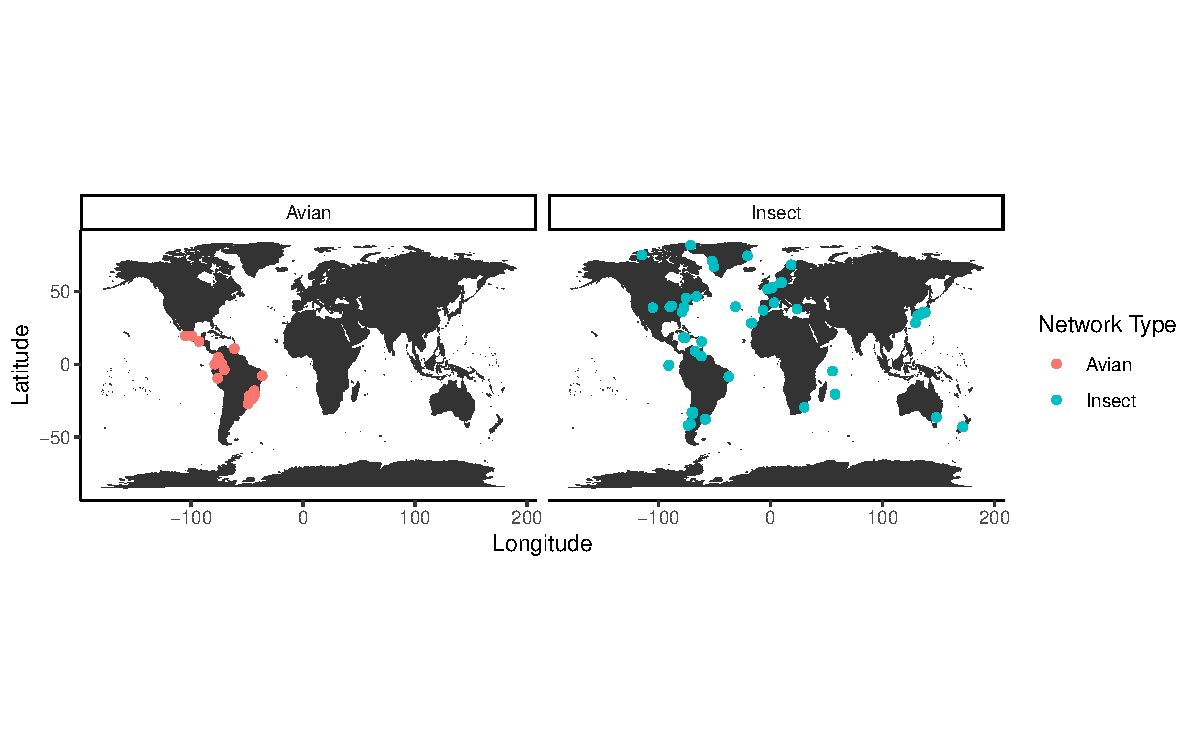
\includegraphics[width=\textwidth]{centralRange/figs/pdf/sup/sitemap.pdf}
    \caption[Map of networks used in Chapter 3]{Map of networks used in our study. Each point represents a unique local network, created by observing avian (Red, N=31), or insect (Blue, N=66) floral visitations.}
    \label{fig:S1}
  \end{center}
\end{figure}
\newpage

\begin{figure}[h!]
  \begin{center}
    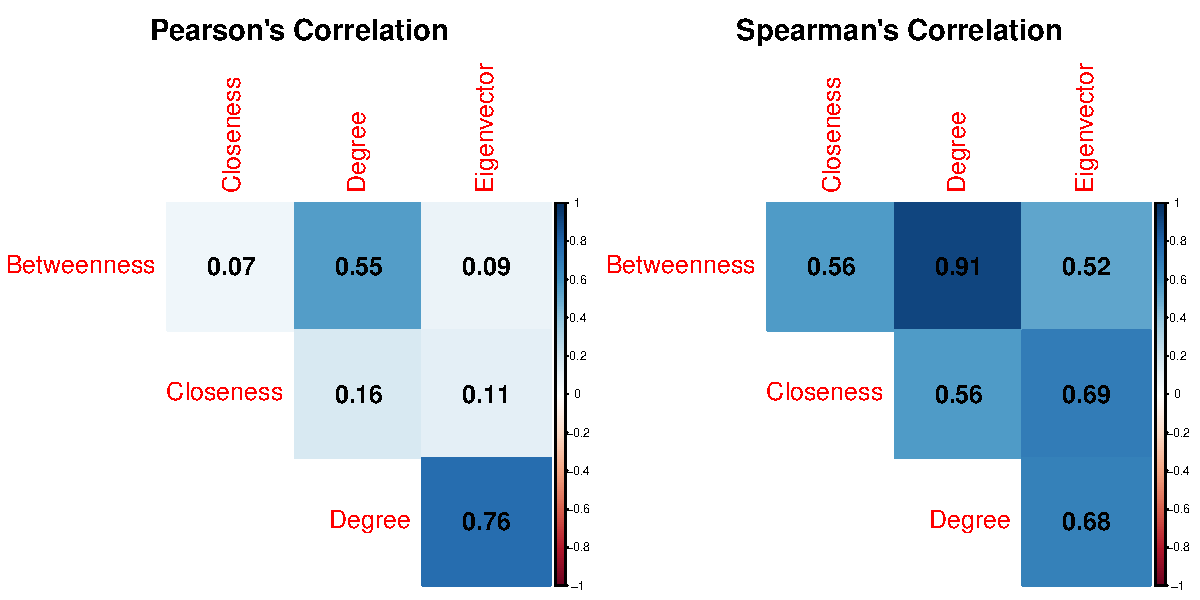
\includegraphics[width=\textwidth]{centralRange/figs/pdf/sup/CentralityCorrelations.pdf}
    \caption[Pairwise correlations of common centrality metrics]{Pairwise correlation of common centrality measure as applied to our global metawebs. While the pearson's correlation of most measures are only slightly positive, spearman's rank correlation shows the ordering of nodes according to alternative measure is relatively conserved. In maintext we present results of closeness centrality, a middle-ground between hyper-local and hyper-global measures.}
    \label{fig:S2}
  \end{center}
\end{figure}

Species that occur in multiple local webs may exhibit different centrality values, dependent both on the compositions and connections observed within any given local community. For species that occur in multiple webs of our dataset, we attempt to predict mean $z-$transformed centrality across all webs where a species is found. To show the variability species may exhibit across networks, we plot the distributions of closeness centrality for species that occur at the most sites across our dataset. Differences between raw and z-standardized metaweb centrality stem from the number of couccuring extraguild partner species. Narrow-ranged plants that cooccur a small set of potential pollinator species are less likely to be highly central in the global metaweb, regardless of local connectivity. We show the relationship between geographic range size and the number of extraguild cooccuring species in \ref{fig:S4}. 


\begin{figure}[h!]
  \begin{center}
    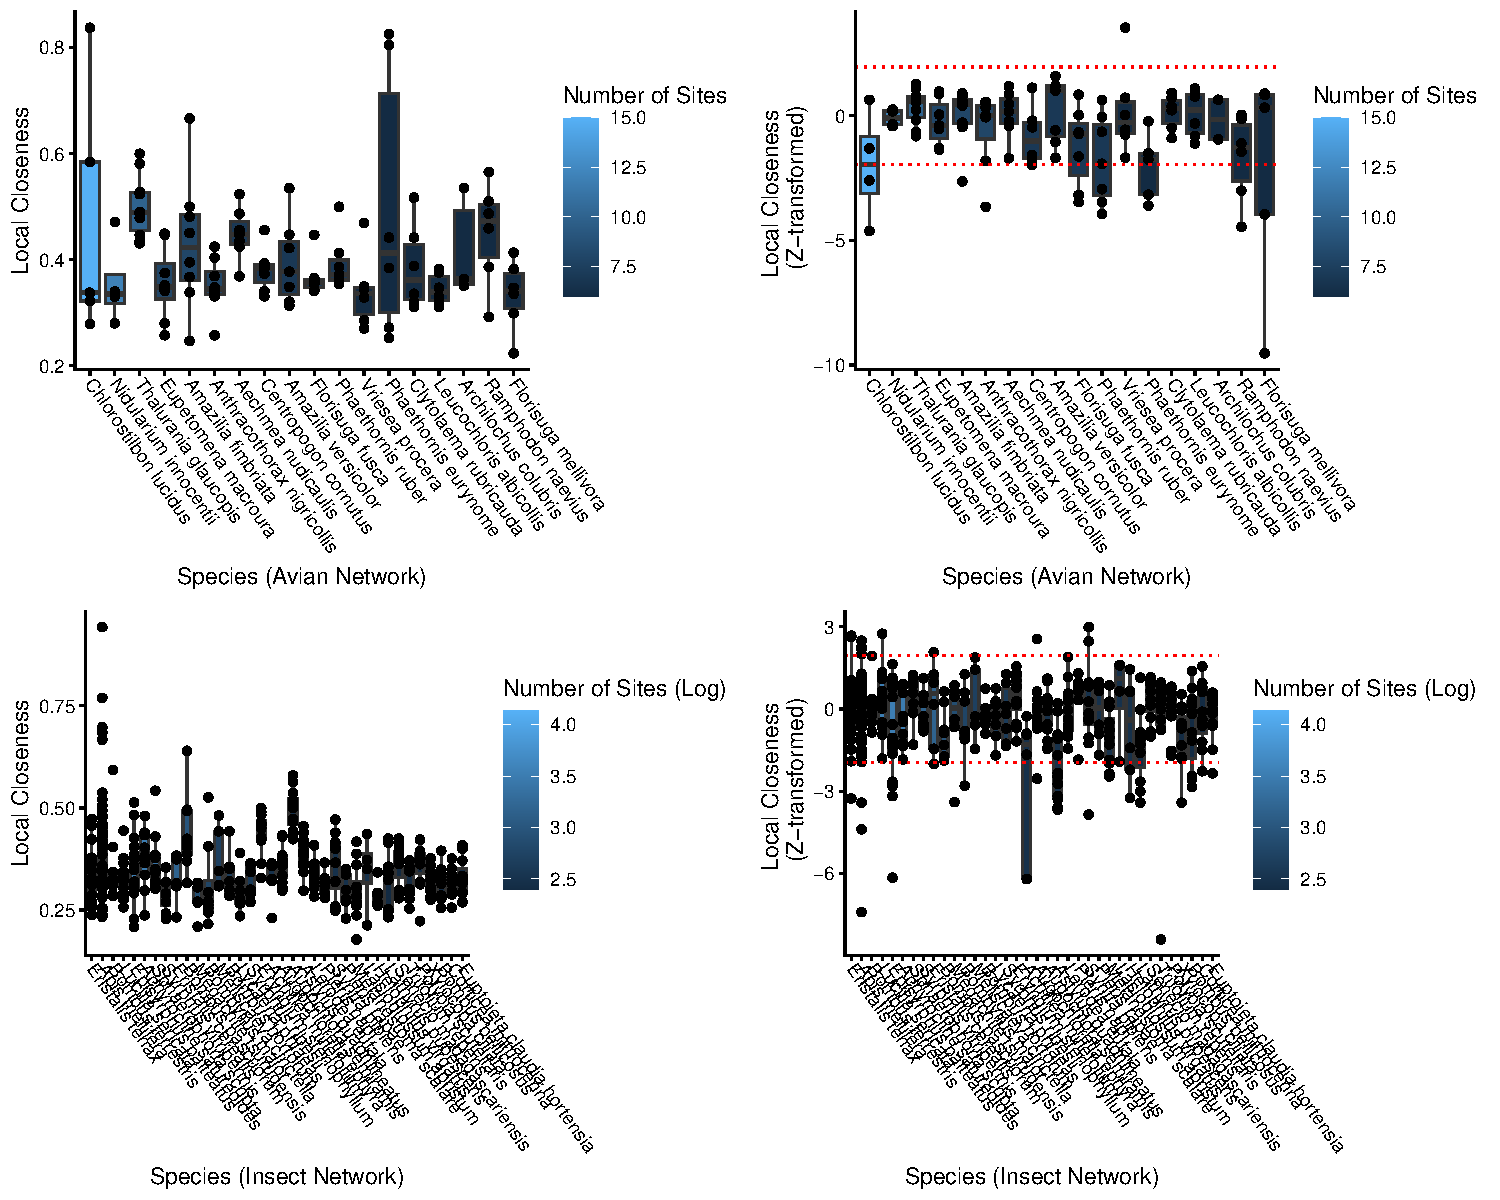
\includegraphics[width=\textwidth]{centralRange/figs/pdf/sup/Local_Centrality_Distributions.pdf}
    \caption[Distribution of local closeness centrality]{Distribution of closeness centrality in local networks for species that occur at multiple sites. Top row of plots represent nodes in bird-plant networks with 7 or more occurrences. Bottom row represent nodes in insect-plant networks with 11 or more occurrences. Left columns represent unstandardized local closeness centrality values. Right column represents the same points after z-score standardization with respect to 1000 null model randomization (see text).}
    \label{fig:S3}
  \end{center}
\end{figure}

\begin{figure}[h!]
\centering
    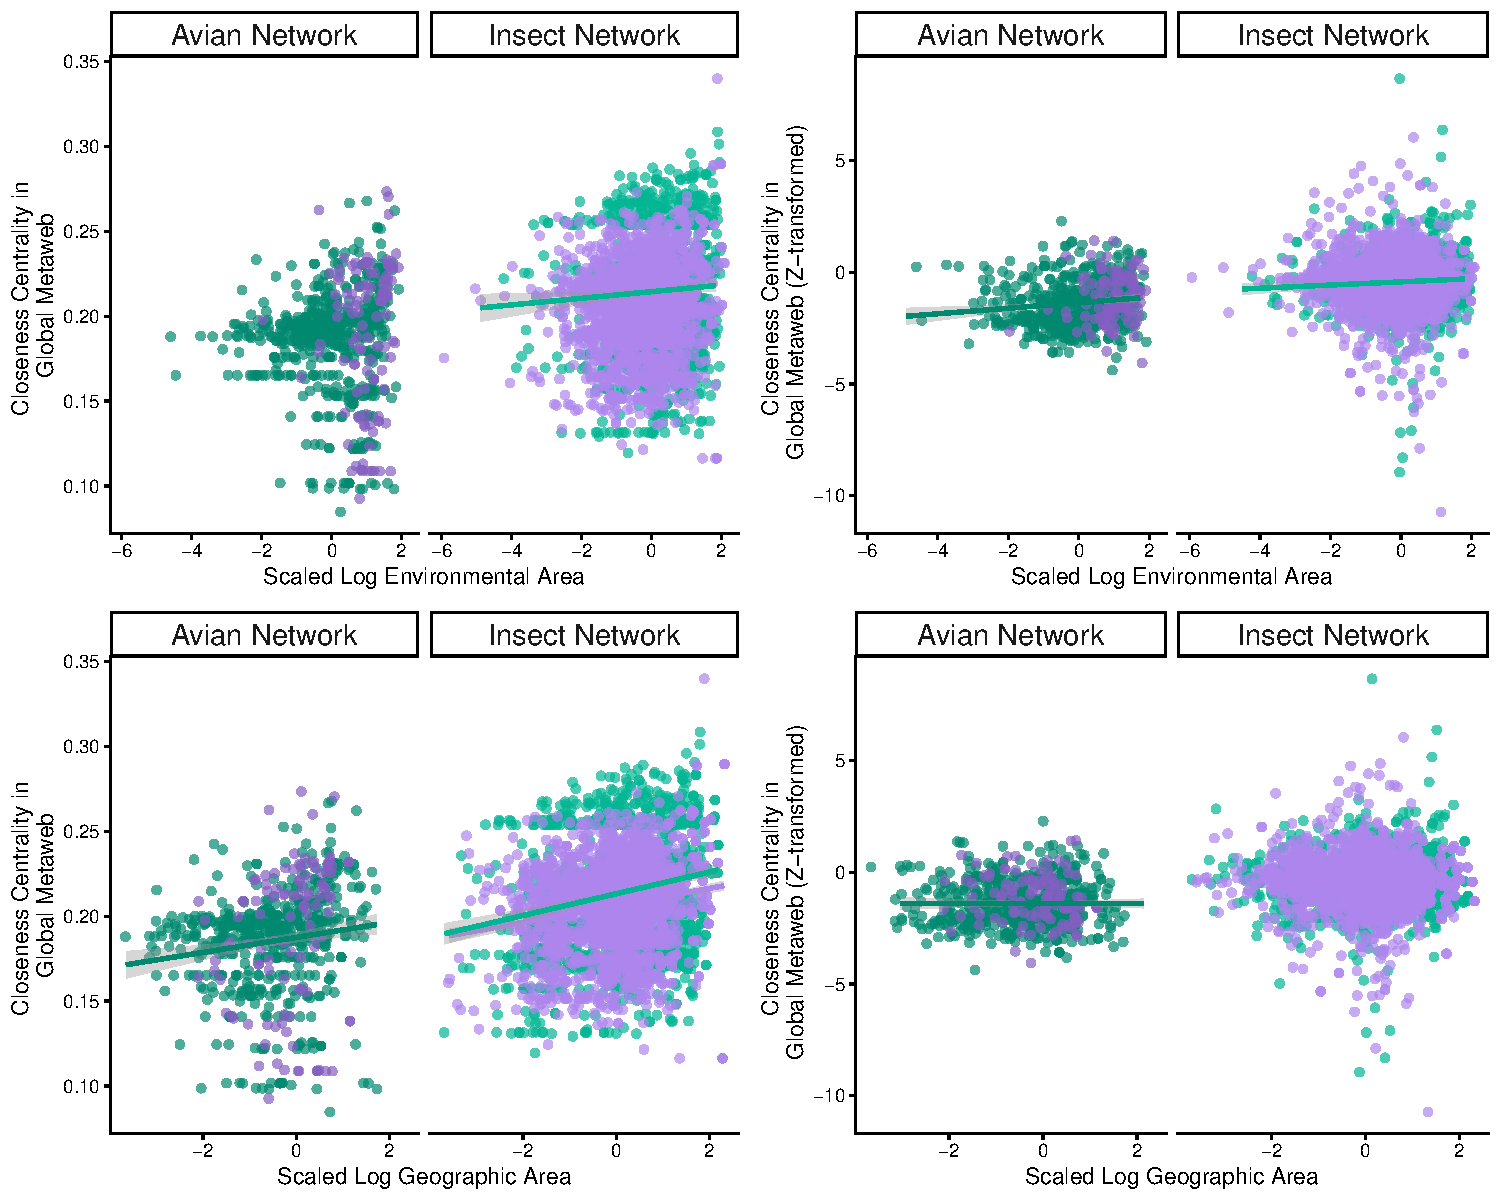
\includegraphics[width=\columnwidth]{centralRange/figs/pdf/sup/MetawebCentralityPlot.pdf}%
    \caption[Species-level closeness centrality in the global metaweb as a function of  environmental niche breadth or geographic range size]{Species-level closeness centrality in the global metaweb as a function of  environmental niche breadth (A,C) or geographic range size (B,D). Plots in the left column show observed centrality values(A,B), while those in the right column show $z-$transformed centrality values based on permutations of local networks(C,D). Points and line colors respond to plant (green) or floral visitor (purple) nodes, respectively. Colored lines depict linear relationships between variables with $POP_2$ values $<0.05$ in our Bayesian GLMs (included for illustrative purposes only).}
    \label{fig:metawebScale}
\end{figure}



\begin{figure}[h!]
  \begin{center}
    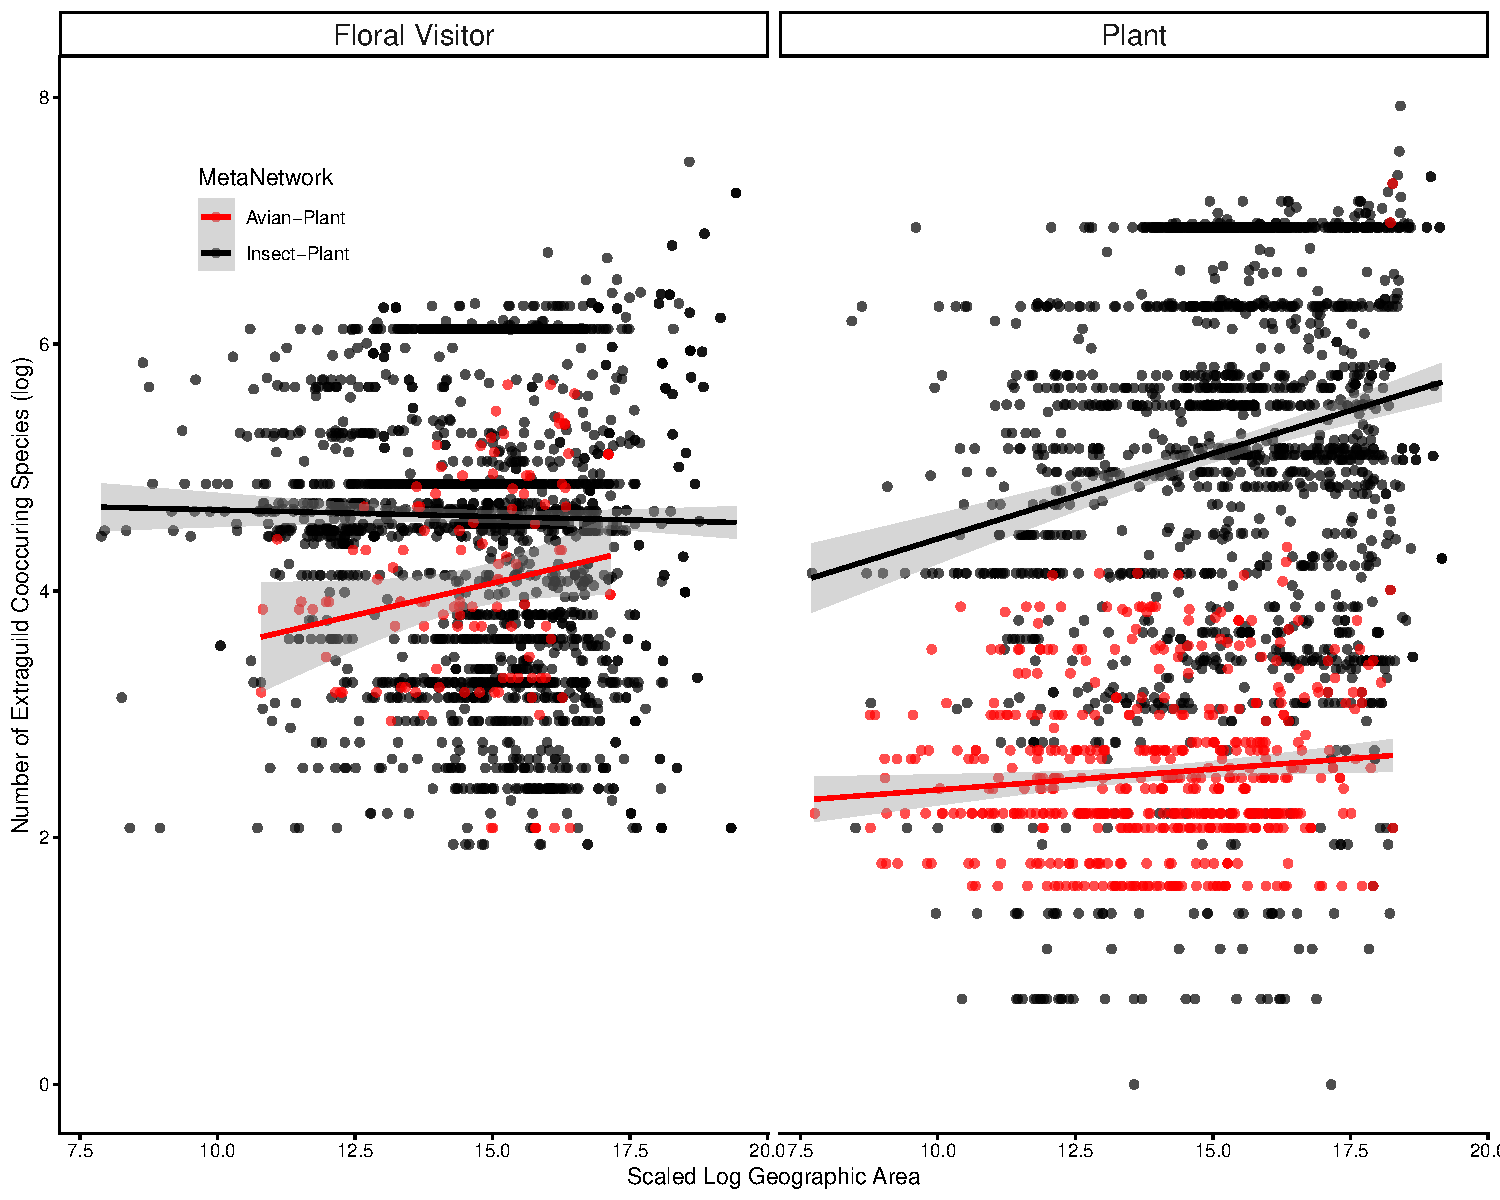
\includegraphics[width=\textwidth]{centralRange/figs/pdf/sup/Cooccurence_vs_GeographicRange.pdf}
    \caption[Relationship between log geographic range size and number of potential partners]{Relationship between log geographic range size (x-axis), and number of potential partners (extraguild species) it cooccurs with in our dataset. Shaded lines represent 95\% confidence intervals of a linear model. For insect-pollinated plants, we see a significant positive relationship between a species' geographic range size and the diversity of insect species it coocures with alongside its range (alpha, p). We see no significant effect of range size on potential interactor richness for avian-pollinated plants, or either pollinator group}
    \label{fig:S4}
  \end{center}
\end{figure}

\begin{figure}[h!]
  \begin{center}
    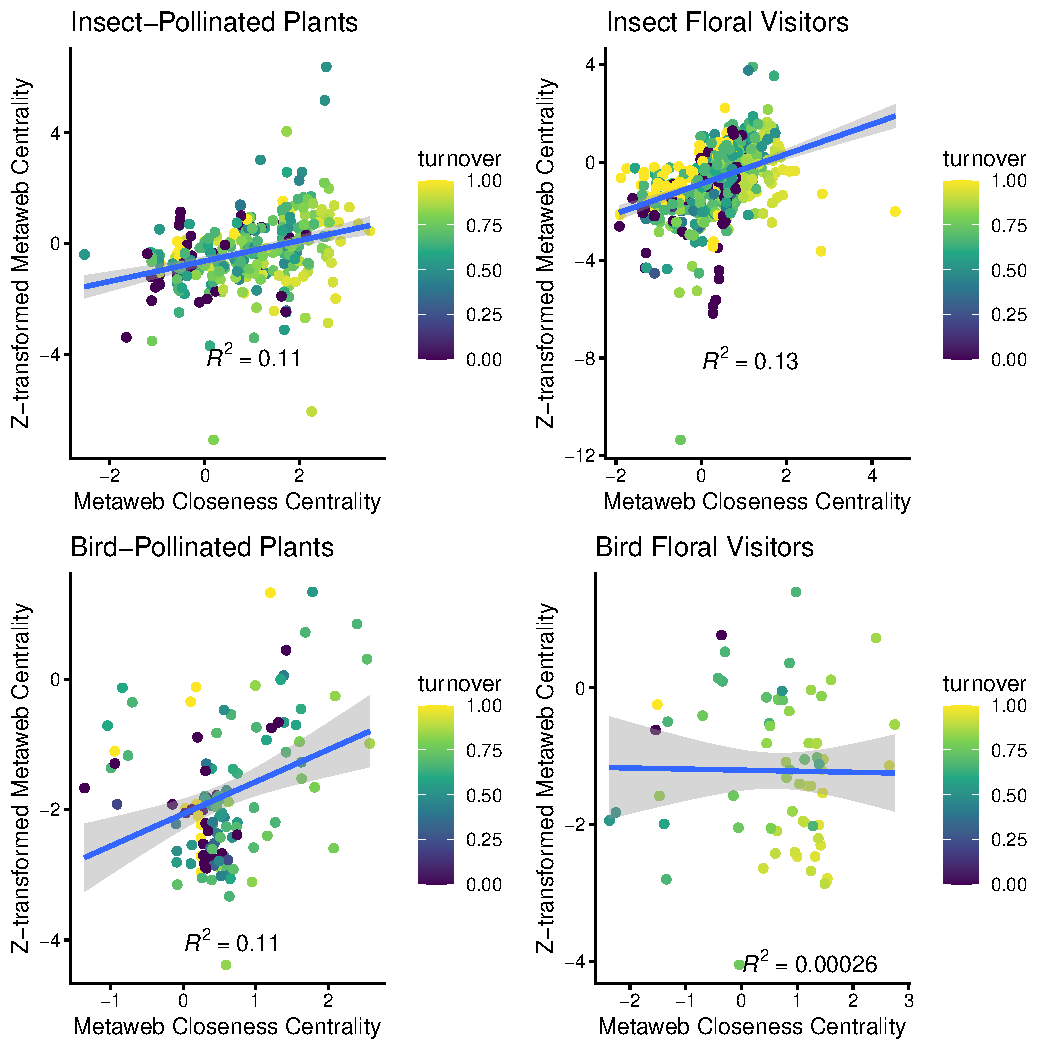
\includegraphics[width=\textwidth]{centralRange/figs/pdf/sup/closenesscomparison.pdf}
    \caption[Comparison of unstandardized and z-standardized closeness centrality]{Comparison of unstandardized (x-axis) and z-standardized (y-axis) closeness centrality in global metawebs across our four node types. Points are colored by interaction turnover across sites. While there is a weak positive relationship between our centrality measure across most node types, the lack of strong explanatory power indicated that our z-transformation procedure does indeed capture alternative aspects of node connectivity at the metaweb scale.}
    \label{fig:S5}
  \end{center}
\end{figure}

\clearpage
Below we present diagnostic pairs plots of all bayesian multivariate regression models presented in the main text. Despite a positive correlation between log geographic range size and log environmental range area (Pearson's $r=0.56$) and negative correlation between fit slope values in some models, correlation structure did not prevent effective inference or MCMC chain convergence ($\hat{R}$ <1.01 across all presented models). 
\begin{figure}[h!]
  \begin{center}
    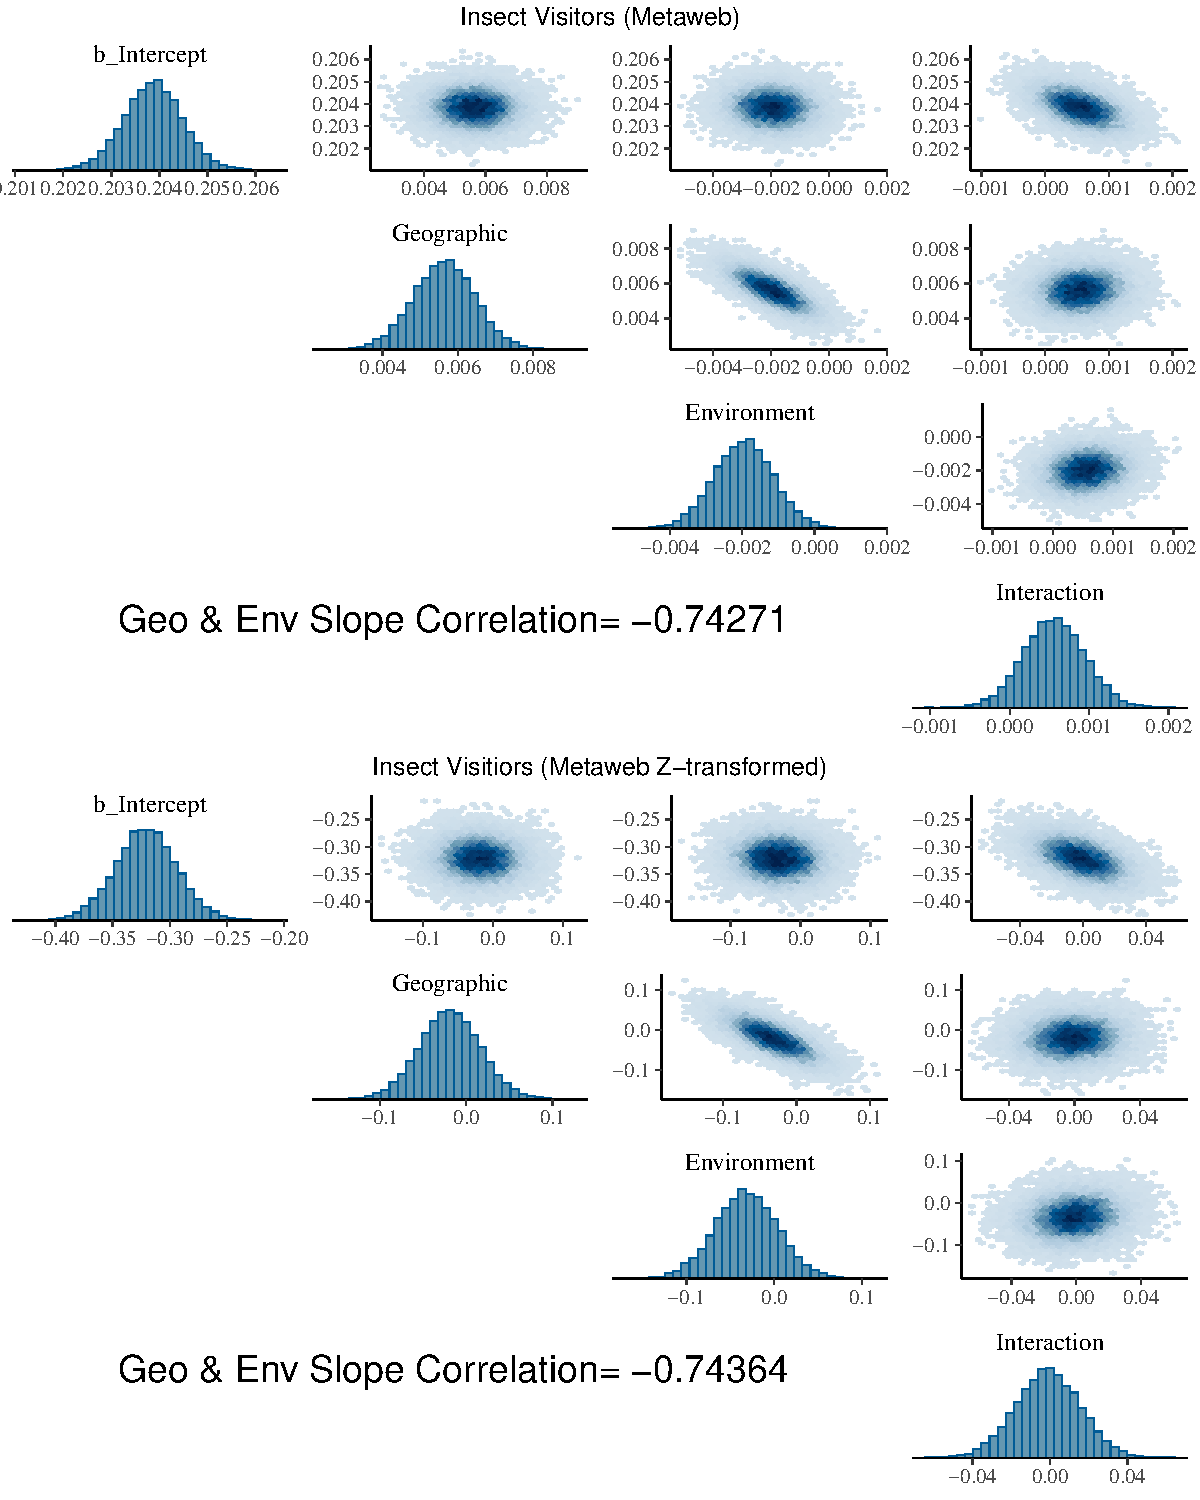
\includegraphics[width=0.8\textwidth]{centralRange/figs/pdf/sup/Pairplot_Insect_Visitors_Metaweb.pdf}
    \caption[Global Closeness centrality pairsplots of floral visitors]{Pairs plots of fit slope and intercept parameters for models of closeness centrality of \textbf{insect floral visitors} in the \textbf{global metaweb}. Hex plots represent the bivariate density of parameter estimates sampled from the posterior, while histograms represent univariate densities of each parameter. Top plots represent a model using raw closeness centrality values as a response variable; lower plots represent a model predicting z-standardized centrality. While there is some negative slope correlation between slope parameters for niche breadth and geographic range, observed $\hat{R}$ values <1.01 indicate adequate chain convergence for inference.}    \label{fig:S6}
  \end{center}
\end{figure}

\begin{figure}[h!]
  \begin{center}
    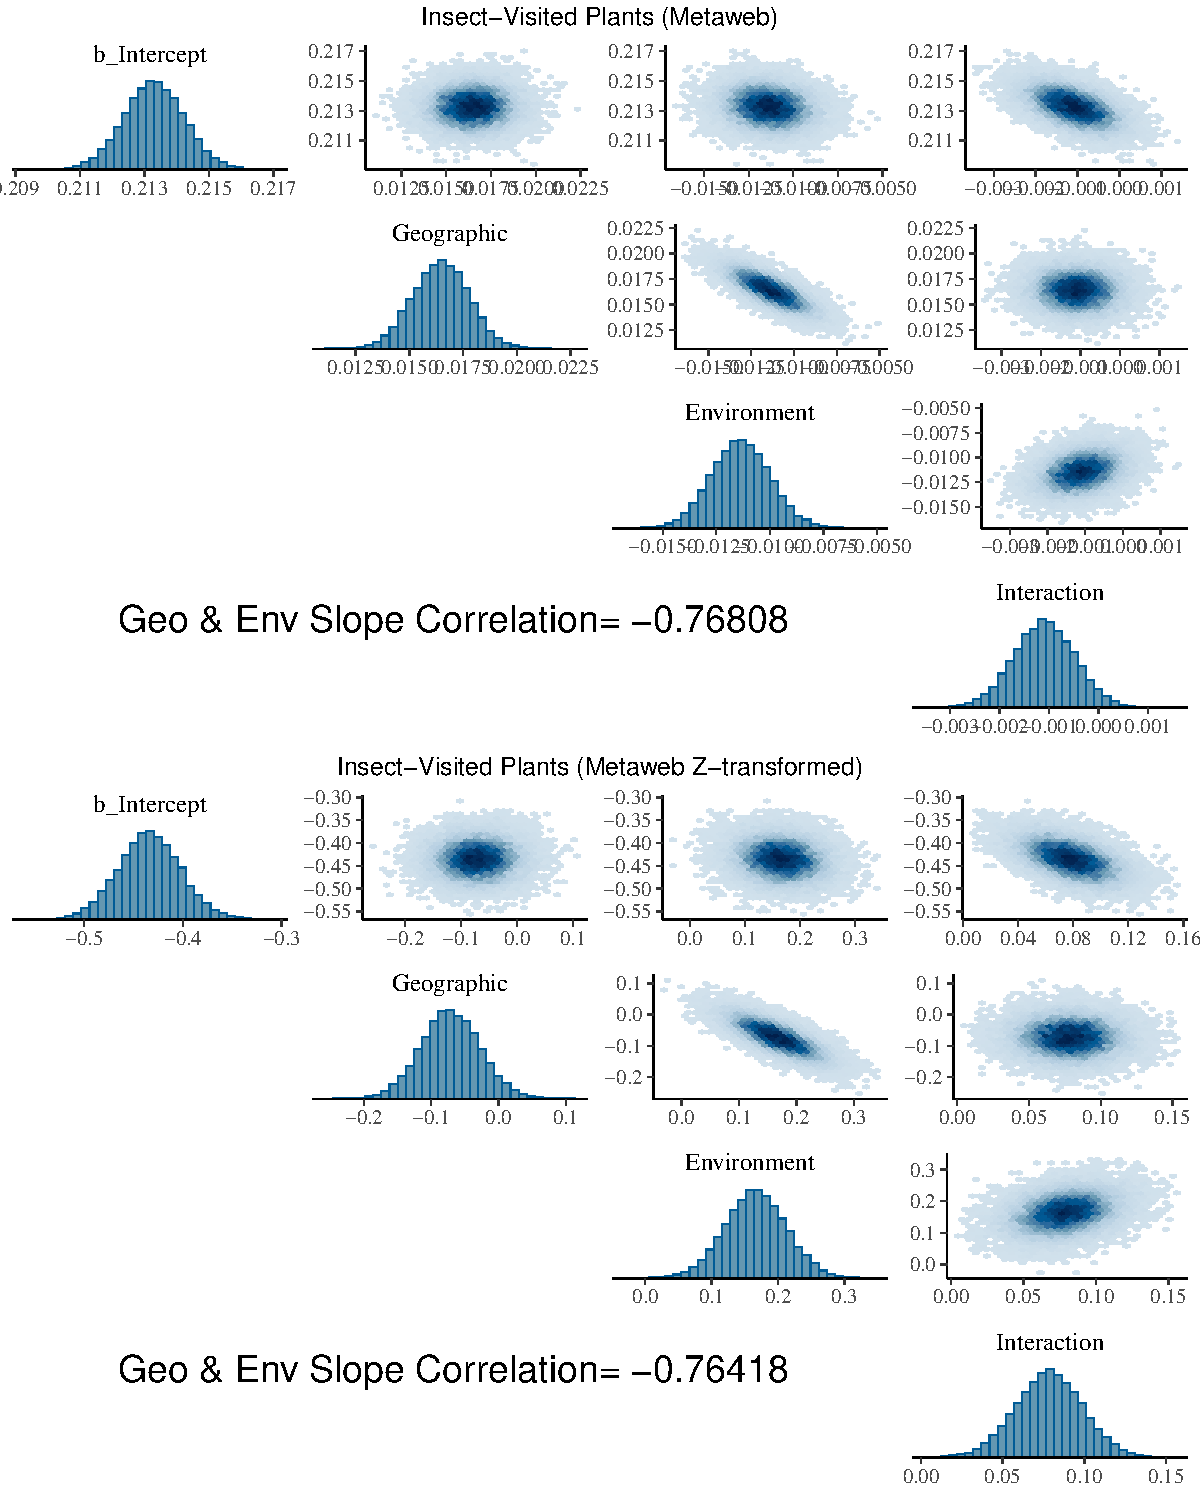
\includegraphics[width=0.8\textwidth]{centralRange/figs/pdf/sup/Pairplot_Insect_Plants_Metaweb.pdf}
    \caption[Global closeness centrality pairsplots of insect-visited plants]{Pairs plots of fit slope and intercept parameters for models of closeness centrality of \textbf{insect-visited plants} in the \textbf{global metaweb}. Hex plots represent the bivariate density of parameter estimates sampled from the posterior, while histograms represent univariate densities of each parameter. Top plots represent a model using raw closeness centrality values as a response variable; lower plots represent a model predicting z-standardized centrality. While there is some negative slope correlation between slope parameters for niche breadth and geographic range, observed $\hat{R}$ values <1.01 indicate adequate chain convergence for inference.}
    \label{fig:S7}
  \end{center}
\end{figure}

\begin{figure}[h!]
  \begin{center}
    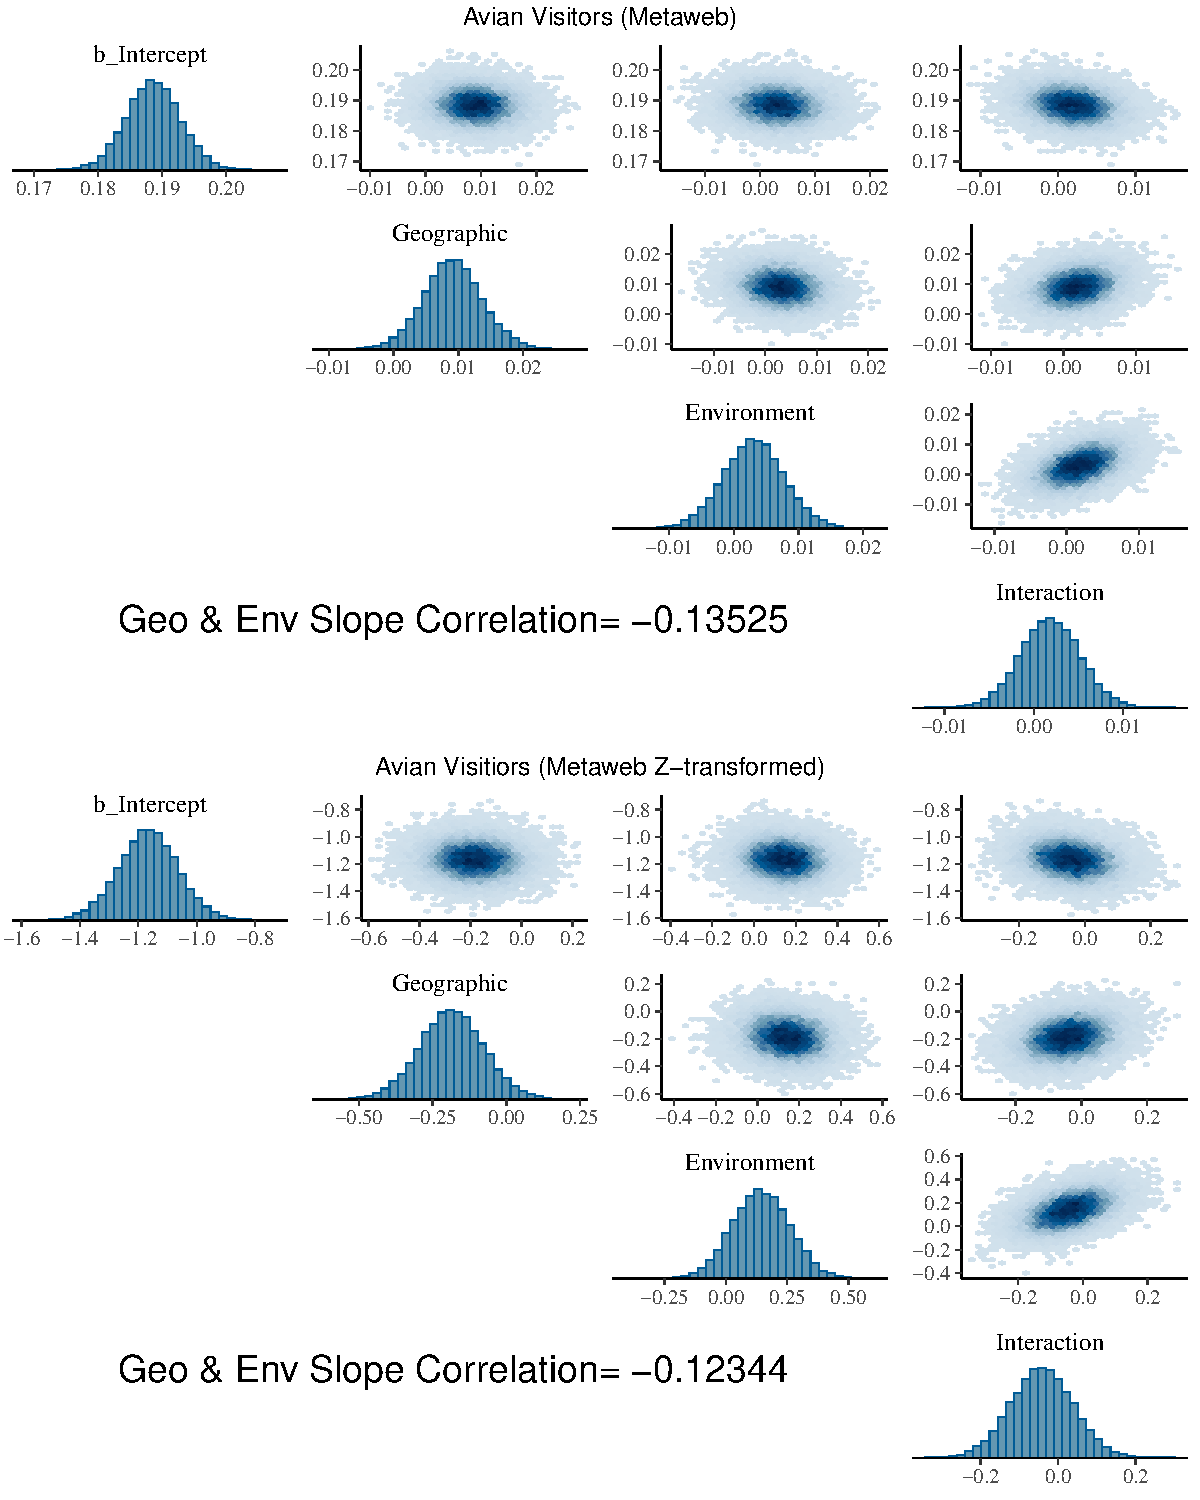
\includegraphics[width=0.8\textwidth]{centralRange/figs/pdf/sup/Pairplot_Avian_Visitors_Metaweb.pdf}
    \caption[Global closeness centrality pairsplots of avian floral visitors]{Pairs plots of fit slope and intercept parameters for models of closeness centrality of \textbf{avian floral visitor} in the \textbf{global metaweb}. Hex plots represent the bivariate density of parameter estimates sampled from the posterior, while histograms represent univariate densities of each parameter. Top plots represent a model using raw closeness centrality values as a response variable; lower plots represent a model predicting z-standardized centrality.}
    \label{fig:S8}
  \end{center}
\end{figure}

\begin{figure}[h!]
  \begin{center}
    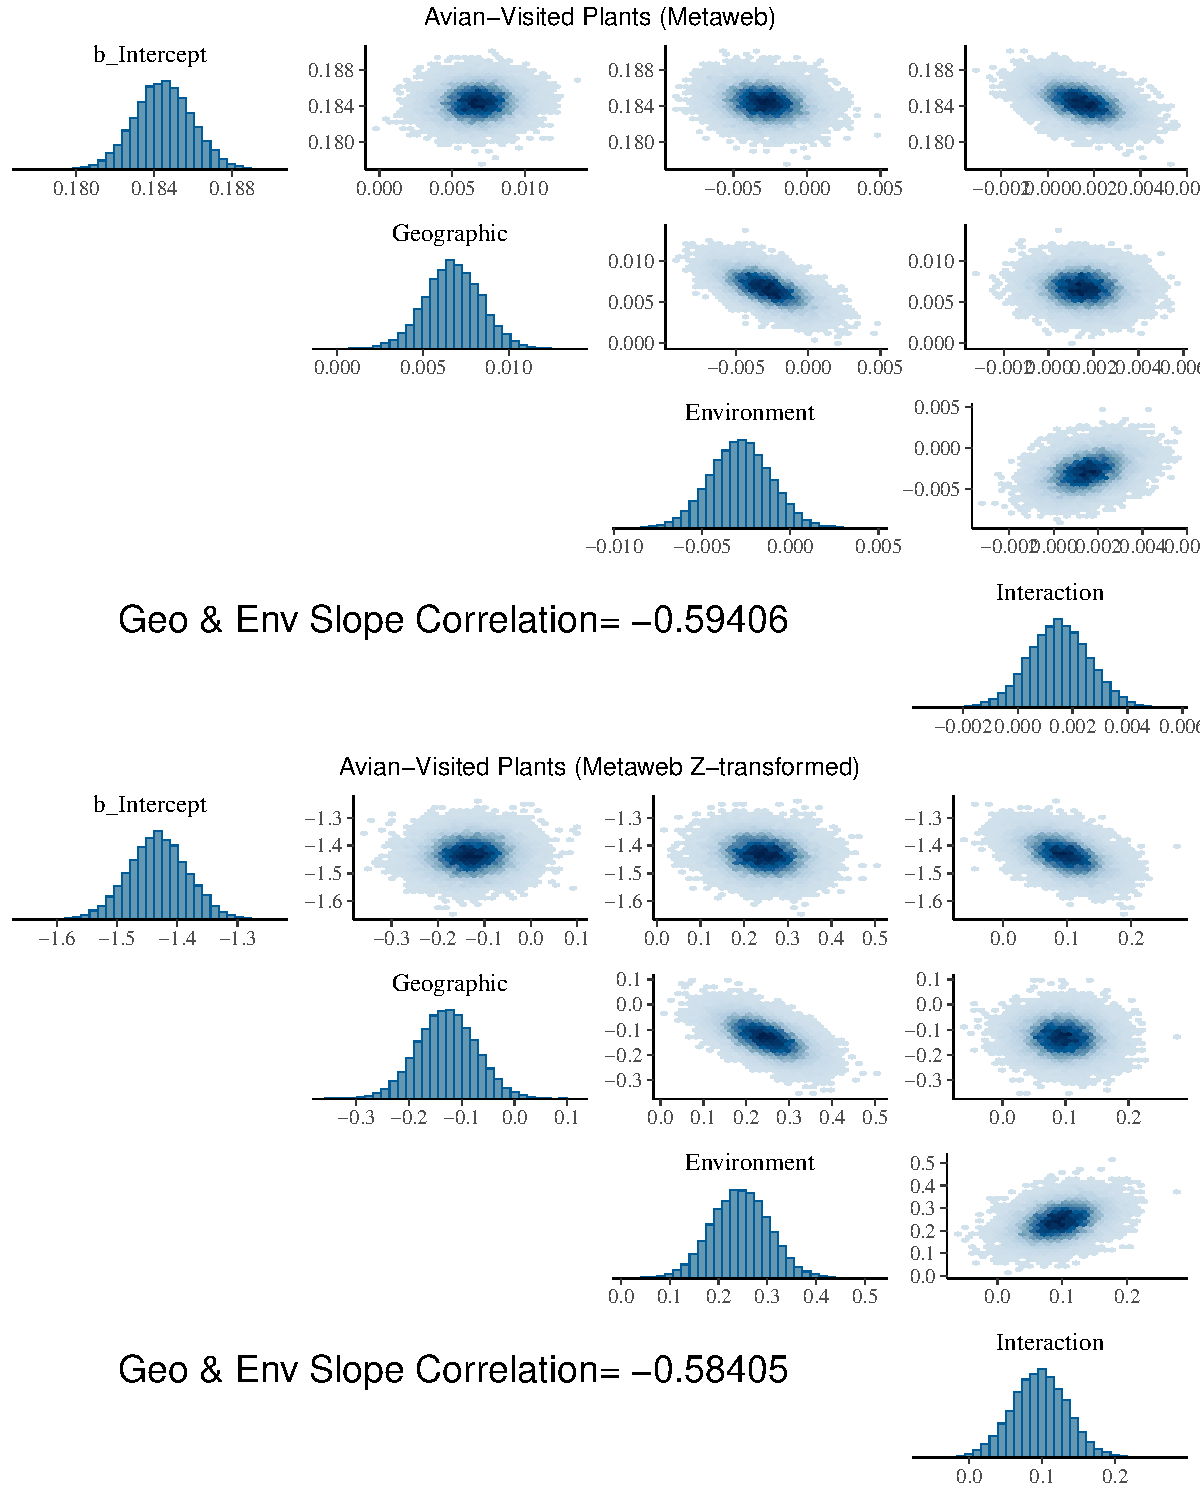
\includegraphics[width=0.8\textwidth]{centralRange/figs/pdf/sup/Pairplot_Avian_Plants_Metaweb.pdf}
    \caption[Global closeness centrality pairsplots of avian-visited plants]{Pairs plots of fit slope and intercept parameters for models of closeness centrality of \textbf{avian-visited plants} in the \textbf{global metaweb}. Hex plots represent the bivariate density of parameter estimates sampled from the posterior, while histograms represent univariate densities of each parameter. Top plots represent a model using raw closeness centrality values as a response variable; lower plots represent a model predicting z-standardized centrality. While there is some negative slope correlation between slope parameters for niche breadth and geographic range, observed $\hat{R}$ values <1.01 indicate adequate chain convergence for inference.}
    \label{fig:S9}
  \end{center}
\end{figure}


\begin{figure}[h!]
  \begin{center}
    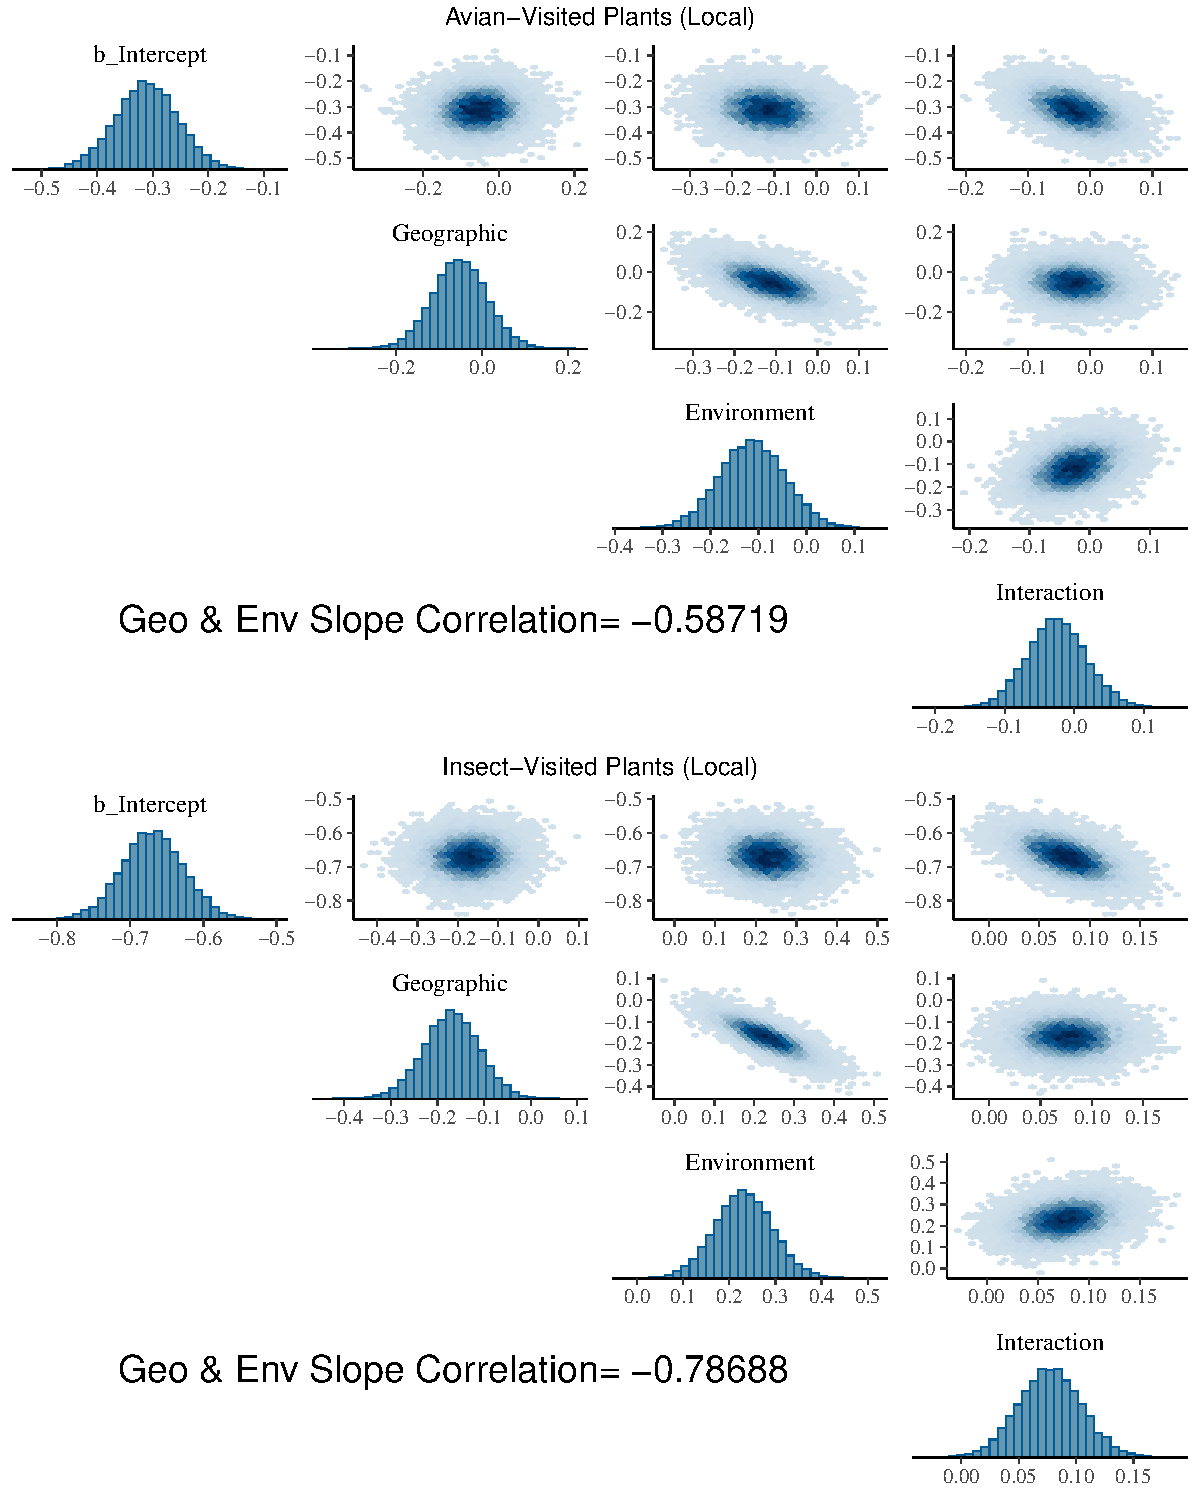
\includegraphics[width=0.8\textwidth]{centralRange/figs/pdf/sup/Pairplot_Plants_Local.pdf}
    \caption[Closeness centrality pairsplots of plants in the local webs]{Pairs plots of fit slope and intercept parameters for models of closeness centrality of \textbf{plants} in \textbf{local webs}. Hex plots represent the bivariate density of parameter estimates sampled from the posterior, while histograms represent univariate densities of each parameter. Top plots represent plants in avian-plant networks; lower plots represent plants in insect-plant networks. While there is some negative slope correlation between slope parameters for niche breadth and geographic range, observed $\hat{R}$ values <1.01 indicate adequate chain convergence for inference.}
    \label{fig:S10}
  \end{center}
\end{figure}

\begin{figure}[h!]
  \begin{center}
    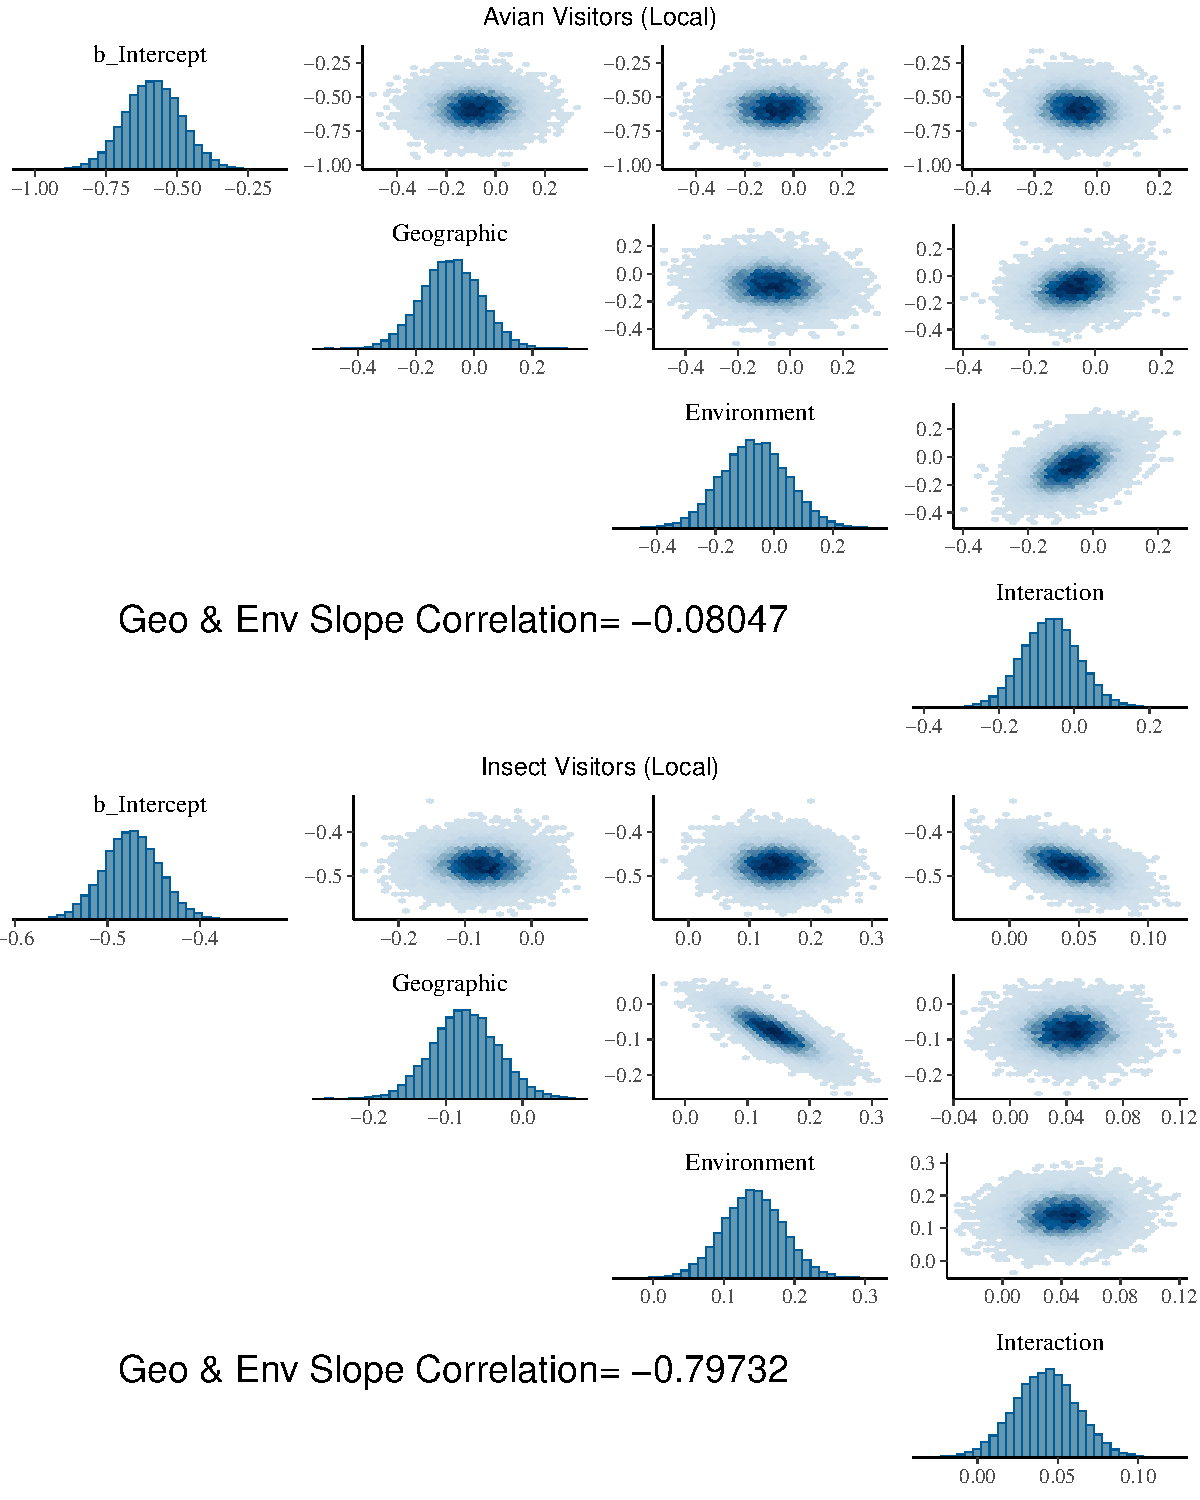
\includegraphics[width=0.8\textwidth]{centralRange/figs/pdf/sup/Pairplot_Visitors_Local.pdf}
    \caption[Closeness centrality pairsplots of floral visitors in the local webs]{Pairs plots of fit slope and intercept parameters for models of closeness centrality of \textbf{floral visitors} in \textbf{local webs}. Hex plots represent the bivariate density of parameter estimates sampled from the posterior, while histograms represent univariate densities of each parameter. Top plots represent birds in avian-plant networks; lower plots represent insects in insect-plant networks. While there is some negative slope correlation between slope parameters for niche breadth and geographic range in the model of local insect visitors, observed $\hat{R}$ values <1.01 indicate adequate chain convergence for inference.}
    \label{fig:S11}
  \end{center}
\end{figure}
